% ============================================================
% v4 演示波④ · 衔接预备（§1.2.1 空间中的点、直线与空间向量）
% 件型依据：交接-20260907b§五（衔接预备件：学前衔接·补前序·必会题——补讲条目＋衔接必会题）；
%   题源＝衔接29全文.txt §1.2.1（知识点条目 1.2.1-1／1.2.1-3 挖空化；题 1.2.1.1-1／1.2.1.2-6 逐字）。
% 版式＝样张v4/导学件 竖放双栏惯用法拷贝改造：A4 竖放四边 15mm、双栏 86.25mm 无栏线、
%   正文 10.5pt/18pt、\linespread{1}＋\raggedcolumns、页脚左章名小字＋右 DDDDDD 灰块页码
%   底缘离底 ≈11mm、题号悬挂 7mm、题后紧跟【答案】（拍板12 同构）、挖空 15mm、纯灰阶 黑＋777777＋DDDDDD。
% 衔接件差异（登记）：课时标题 \keshi 14pt 居中；◆知识点块（\zsd 同款）；题号「衔接N．」自定义宏
%   hang 7mm、无难度侧标（不区分难度口径）；知识点条目悬挂同 7mm（撤导学件条目 1.6em）；
%   知识点条目源图不随迁（补讲图回填债登记）；题图全 TikZ 重绘（源图不随迁）；
%   答案值 \dfrac、详解内 \frac；点拨 并入详解段末接排（{\heiti 点拨} 引导，逐字）。
% 编译：xelatex main.tex（两遍）→ render.py（先清 png/）→ 断言题号列.py＋断言版式.py
% ============================================================
\documentclass[fontset=none]{ctexart}

% ---------- 字体（同导学件 v4） ----------
\setmainfont{Times New Roman}
\setCJKmainfont[BoldFont=SimHei]{SimSun}
\setCJKfamilyfont{hei}{SimHei}
\setCJKfamilyfont{kai}{KaiTi}
\newcommand{\heiti}{\CJKfamily{hei}}
\newcommand{\kaishu}{\CJKfamily{kai}}
\xeCJKDeclareCharClass{CJK}{"2460->"24FF, "2600->"26FF, "2200->"22FF, "25A0->"25FF}
\xeCJKsetup{CheckSingle=true}

% ---------- 宏包 ----------
\usepackage[a4paper,margin=15mm,headheight=12pt,headsep=2mm,footskip=13pt]{geometry}
\usepackage{amsmath,amssymb}
\usepackage{graphicx}
\usepackage{xcolor}
\usepackage{multirow,array,calc}
\usepackage{multicol}
\usepackage{needspace}
\usepackage{fancyhdr}
\usepackage{tcolorbox}
\usepackage{tikz}

% ---------- 颜色（黑＋777777＋DDDDDD） ----------
\definecolor{midgray}{HTML}{777777}
\definecolor{pnumbg}{HTML}{DDDDDD}

% ---------- 版面（竖放双栏，同导学件 v4） ----------
\setlength{\columnsep}{7.5mm}
\setlength{\columnseprule}{0pt}
\setlength{\multicolsep}{3pt}
\renewcommand{\normalsize}{\fontsize{10.5pt}{18pt}\selectfont}
\linespread{1}
\normalsize
\setlength{\parindent}{2em}
\clubpenalty=10000
\widowpenalty=10000
\displaywidowpenalty=10000
\tolerance=9999
\emergencystretch=8em
\binoppenalty=100
\relpenalty=100
\flushbottom
\raggedcolumns

\setlength{\arrayrulewidth}{0.4pt}
\setlength{\tabcolsep}{3pt}
\renewcommand{\arraystretch}{1.15}

% ---------- 页脚（左章名小字＋右灰块页码，底缘离页底≈11mm，同导学件 v4） ----------
\pagestyle{fancy}
\fancyhf{}
\renewcommand{\headrulewidth}{0pt}
\fancyfoot[L]{\fontsize{6.5pt}{8pt}\selectfont\color{midgray}第1章\ 空间向量与立体几何\ ·\ 衔接预备}
\fancyfoot[R]{\raisebox{0.59mm}[0pt][0pt]{\setlength{\fboxsep}{0pt}\colorbox{pnumbg}{\makebox[31mm][c]{\rule{0pt}{5mm}\fontsize{10.5pt}{12pt}\selectfont\bfseries\thepage}}}}

% ---------- 标题命令 ----------
% 课时标题：14pt 黑体居中（同导学件 \keshi）
\newcommand{\keshi}[1]{\par\Needspace*{3\baselineskip}\addvspace{3pt}%
  {\centering\fontsize{14pt}{20pt}\selectfont\heiti #1\par}\addvspace{2pt}}

% ---------- 正文宏（multicols 内：防孤悬一律 \glueguard） ----------
\newcommand{\glueguard}[1]{\vskip 0pt plus #1\baselineskip\penalty-100\vskip 0pt plus -#1\baselineskip}
\newcommand{\biaoqian}[1]{{\heiti #1}}
\newcommand{\kongbai}{\underline{\hspace*{15mm}}}
\newcommand{\ansul}[1]{\underline{#1}}
% 花形行（板块头，通栏语义在双栏页内以栏内块呈现＝导学件惯用法；底线黑，拍板27）
\newcommand{\huaxing}[2]{\par\glueguard{2}\addvspace{4pt}%
  \noindent{\tcbox[on line,colback=white,colframe=black,boxrule=0.5pt,arc=2.5mm,%
    left=5pt,right=5pt,top=1.5pt,bottom=1.5pt]{\fontsize{12pt}{16pt}\selectfont\heiti #1}}%
  \hfill\raisebox{1pt}{\fontsize{6.5pt}{8pt}\selectfont\color{midgray}#2}\par
  \vspace{1.5pt}\noindent{\color{black}\rule{80mm}{0.8pt}}\par\addvspace{3pt}}
% 知识点标题：◆ 知识点N｜名（12pt 黑体，同导学件 \zsd 惯用法）
\newcommand{\zsd}[2]{\par\glueguard{4}\addvspace{3pt}%
  \noindent{\fontsize{12pt}{17pt}\selectfont\bfseries ◆\ 知识点#1\quad #2}\par\addvspace{2pt}}
% 知识点条目（悬挂 7mm＝题号列口径统一，撤导学件条目 1.6em——衔接件差异登记）
\newcommand{\knitem}[1]{\par\glueguard{1}\noindent\hangindent=7mm\hangafter=1 #1\par}
% 衔接题号（hang 7mm、无难度侧标——不区分难度口径）
\newcommand{\xtian}[2]{\par\glueguard{4}\addvspace{2pt}%
  \noindent\hangindent=7mm\hangafter=1{\heiti #1}#2\par}
% 【答案】行（整体缩进 7mm；值 \ansul 显式逐值包）
\newcommand{\ansline}[1]{\par\glueguard{2}\noindent\hangindent=7mm\hangafter=0\biaoqian{【答案】}#1\par}
% 题图块（TikZ 矢量，30mm 档居中，从题号右缘 7mm 起排；显式清零悬挂残留）
\newcommand{\tikzblk}[1]{\penalty10000\noindent\hangindent=0pt\hangafter=1\hspace*{7mm}%
  \makebox[\dimexpr\linewidth-7mm\relax][c]{#1}\par\penalty10000}

\begin{document}

\begin{multicols}{2}
\raggedcolumns
\emergencystretch=8em

\keshi{1.2.1\ 空间中的点、直线与空间向量}

\huaxing{衔接预备}{学前衔接·补前序·必会题}

\zsd{一}{平行线分线段成比例定理}

\knitem{（1）平行线分线段成比例定理：三条平行线截两条直线，截得的\kongbai{}成比例．}
\knitem{（2）变形：\({\rm A}\)字型、\(8\)字型，其中\(DE \parallel BC\)，则对应线段\kongbai．}

\zsd{二}{射影定理}

\knitem{（1）内容：若\(AB \perp AC\)，\(AD \perp BC\)，则\(BA^{2} = BD \cdot \kongbai\)，\(CA^{2} = \kongbai \cdot CB\)，\(DA^{2} = DB \cdot DC\)．}
\knitem{（2）记忆：\kongbai{}的平方＝\kongbai{}×\kongbai{}．}

\xtian{衔接1．}{如图，在△\(ABC\)中，\(\dfrac{AD}{AB}=\dfrac{1}{4}\)，\(\dfrac{AE}{AC}=\dfrac{1}{2}\)，\(BE\)和\(CD\)相交于点\(F\)，则\(\dfrac{DF}{DC}=\)\kongbai．}

\tikzblk{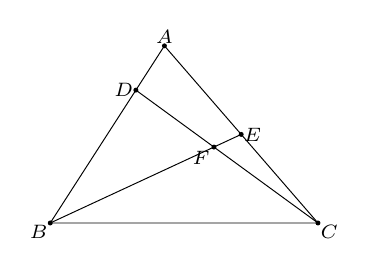
\begin{tikzpicture}[x=1mm,y=1mm,line width=0.35pt,
  every node/.style={font=\fontsize{7.5pt}{8.5pt}\selectfont,inner sep=0.8pt}]
  \coordinate (A) at (14.5,22.5);
  \coordinate (B) at (0,0);
  \coordinate (C) at (34,0);
  \coordinate (D) at (10.875,16.875);
  \coordinate (E) at (24.25,11.25);
  \coordinate (F) at (20.79,9.64);
  \draw (A) -- (B) -- (C) -- cycle;
  \draw (B) -- (E);
  \draw (C) -- (D);
  \foreach \p in {A,B,C,D,E,F} \fill (\p) circle (0.9pt);
  \node[above]       at (A) {$A$};
  \node[below left]  at (B) {$B$};
  \node[below right] at (C) {$C$};
  \node[left]        at (D) {$D$};
  \node[right]       at (E) {$E$};
  \node[below left=0.6pt] at (F) {$F$};
\end{tikzpicture}}

\ansline{\ansul{\(\dfrac{3}{7}\)}}

\noindent\hangindent=7mm\hangafter=0\biaoqian{【分析】}过点\(D\)作\(DG \parallel AC\)交\(BE\)于\(G\)，由平行线分线段成比例把\(DF\)与\(FC\)的比转化为\(DG\)与\(EC\)的比，再由\(AE=EC\)求出\(DF\)与\(DC\)的比．\biaoqian{【详解】}过点\(D\)作\(DG \parallel AC\)交\(BE\)于\(G\)，∵\(\frac{AD}{AB}=\frac{1}{4}\)，∴\(\frac{BD}{AB}=\frac{3}{4}\)，∴\(\frac{DG}{AE}=\frac{3}{4}\)，∵\(\frac{AE}{AC}=\frac{1}{2}\)，∴\(AE=EC\)，∴\(\frac{DG}{EC}=\frac{3}{4}\)，∴\(\frac{DF}{FC}=\frac{3}{4}\)，∴\(\frac{DF}{DC}=\frac{3}{7}\).{\heiti 点拨}\hspace{0.5em}①熟悉\({\rm A}\)字型和\(8\)字型；②涉及到很多线段的比例时，可设元或令其为具体值，比如\(\frac{DF}{FC}=\frac{3}{4}\)，则设\(DF=3k\)，\(FC=4k\)，\(CD=7k \Rightarrow \frac{DF}{DC}=\frac{3k}{7k}=\frac{3}{7}\)；或设\(DF=3\)，\(FC=4\)，\(CD=7 \Rightarrow \frac{DF}{DC}=\frac{3}{7}\).

\xtian{衔接2．}{在Rt△\(ABC\)中，\(\angle BAC=90^{\circ}\)，\(AD \perp BC\)于点\(D\)，若\(\dfrac{AC}{AB}=\dfrac{3}{4}\)，则\(\dfrac{AD}{AC}=\)\kongbai，\(\dfrac{BD}{CD}=\)\kongbai．}

\tikzblk{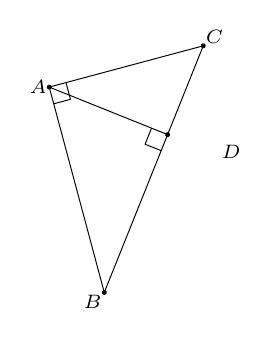
\begin{tikzpicture}[x=1mm,y=1mm,line width=0.35pt,
  every node/.style={font=\fontsize{7.5pt}{8.5pt}\selectfont,inner sep=0.8pt}]
  \begin{scope}[rotate=15]
    \coordinate (A) at (0,27);
    \coordinate (B) at (0,0);
    \coordinate (C) at (20.25,27);
    \coordinate (D) at (12.96,17.28);
    \draw (A) -- (B) -- (C) -- cycle;
    \draw (A) -- (D);
    \draw (0,24.8) -- (2.2,24.8) -- (2.2,27);
    \draw (11.64,15.52) -- (9.88,16.84) -- (11.2,18.6);
    \foreach \p in {A,B,C,D} \fill (\p) circle (0.9pt);
  \end{scope}
  \node[left]        at (-6.99,26.08) {$A$};
  \node[below left]  at (0,0) {$B$};
  \node[above right] at (12.57,31.32) {$C$};
  \node[right]       at (14.6,17.9) {$D$};
\end{tikzpicture}}

\ansline{\ansul{\(\dfrac{4}{5}\)}；\ansul{\(\dfrac{16}{9}\)}}

\noindent\hangindent=7mm\hangafter=0\biaoqian{【分析】}设\(AC=3\)、\(AB=4\)，则\(BC=5\)；先用等积法求斜边上的高\(AD\)，再用射影定理求\(BD\)、\(CD\)．\biaoqian{【详解】}依题意可设\(AC=3\)，\(AB=4\)，则\(BC=5\)，∵\(\frac{AD \cdot BC}{2}=\frac{AB \cdot AC}{2}=6\)，∴\(AD=\frac{12}{5}\)（等积法），∴\(\frac{AD}{AC}=\frac{12}{15}=\frac{4}{5}\)，由射影定理得，\(BA^{2}=BC \cdot BD \Rightarrow BD=\frac{16}{5}\)，\(CA^{2}=CB \cdot CD \Rightarrow CD=\frac{9}{5}\)，∴\(\frac{BD}{CD}=\frac{16}{9}\).{\heiti 点拨}\hspace{0.5em}本题求比值设\(AC=3\)求解简便些，也可采取相似三角形.

\end{multicols}
\end{document}
